\documentclass[12pt,oneside,english]{article}

\usepackage[T1]{fontenc}
\usepackage[latin1]{inputenc}
\usepackage{geometry}
\geometry{verbose,letterpaper,tmargin=1in,bmargin=1in,lmargin=1in,rmargin=1in}
\usepackage{textcomp}
\usepackage{babel}
\setcounter{secnumdepth}{0}
\usepackage{graphicx}
\usepackage{float}
\floatstyle{boxed}
\restylefloat{figure}
\usepackage{longtable}
\usepackage{url}

\newcommand{\BibTeX}{{\sc Bib}\TeX}


\begin{document}
\sffamily

        \title{in-situ impedance and morphology of self-assembling gold nanoislands}

	\author{John Donovan, Dr. Chuhee Kwon\\
	University of California, Long Beach, CA\\
	{\small donovan.csulb@gmail.com ckwon@csulb.edu}}
	
        \date{\today}

	\maketitle


        \section{Introduction}

	\begin{figure}
	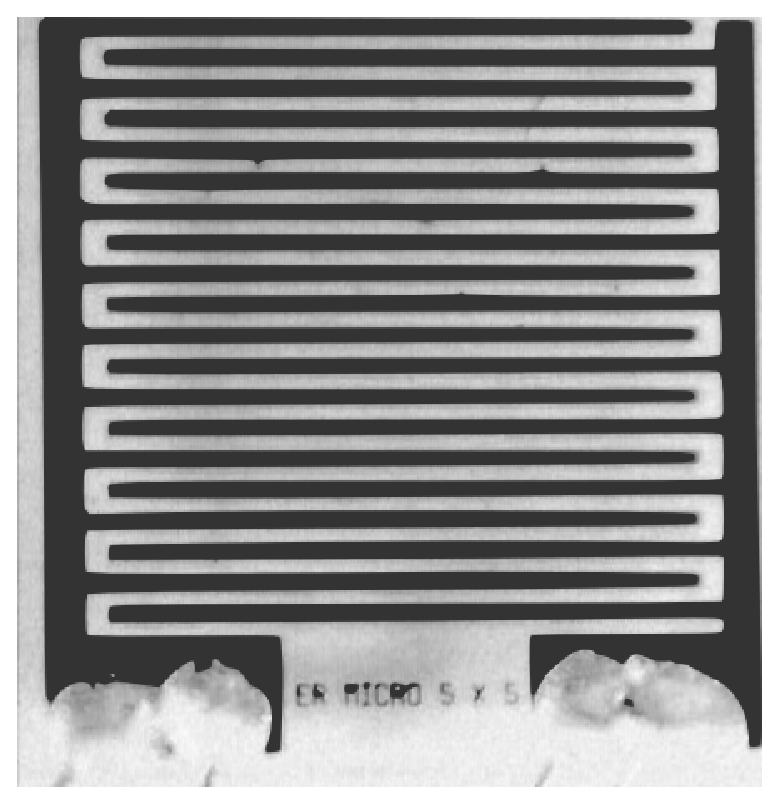
\includegraphics[scale=0.4]{images/IDE.eps} \label{f:IDE}
	\caption{The self-assembling gold monolayers are deposited on a gold inter-digitized electrode (IDE).}
	\end{figure}
	
	\subsection{background}
	Gold nanoislands  are formed by annealing a substrate -- on which gold has been uniformly deposited -- to produce islands within a predictable range of size and shape.
	
	
\begin{quote}
Plasmonic nanoparticles also act as transducers that convert small changes in the local refractive index into spectral shifts in the intense nanoparticle extinction and scattering spectra. 
Most organic molecules have a higher refractive index than buffer solution; 
thus, when they bind to nanoparticles, the local refractive index increases, causing the extinction and scattering spectrum to redshift. 
Molecular binding can be monitored in real time with high sensitivity by using simple and inexpensive transmission spectrometry, which measures extinction, the sum of absorption and scattering 3,8-10,41,42. 
(nature materials | VOL 7 | JUNE 2008 | www.nature.com/naturematerials)
\end{quote}

\begin{quote}
Thus, changes in the local environment - such as through the presence of an adsorbed species - should cause a shift in $\lambda_max$ .
(www.annualreviews.org - Localized Plasmon Spectroscopy
271)
\end{quote}

	\subsection{purpose}
	This research attempts to create reproducible samples of gold nano-islands and study their morphology.
	Prior research suggests that the physical properties of gold nano-islands are sensitive to the method of depositing the gold, the number of layers, and variations in annealing temperature \cite{shon11}.  
	Gold nano-island formation through polymer-assisted self-assembly is also sensitive to the initial size of the colloidal gold used to form the self-assembling layers \\cite(reference), to the temperature profile during annealing, and to the length of time (in days) between creation and annealing (\cite{joshi}).
	This research quantifies the repeatiblity of gold nano-islands produced using the label-free(*) self-assembly method.


	\subsection{method}
	Samples are produced using polymer-assisted self-assembling monolayers.

	\section{Procedure}

	\subsection{The Chemistry of Self-Assembling Films}
	
	\emph{COMMENT: This section is based on discussion with YS Shon, and attribution should be made for these ideas.}
	
	Gold self-assembling films were produced from two sizes of gold particle.  
	The larger particles were Au$_{314}$, the smaller were Au$_{25}$.  
	These particles are coated in different organic ligands, which aid their solubility in ethanol (in the case of Au$_{314}$) and water (in the case of Au$_{25}$).    
	The ligands are terminated with a carboxy group (COOH) in ethanol and aqueous solutions; in the aqueous Au$_{25}$ solution, ligands may also be terminated with a positively charged carboxy group (COO-). 
	
	After the first gold layer is deposited the sample is dipped in an aqueous solution of poly(allyl-amine hydrochloride) (PAH).  
	The PAH bonds to the ligands and allows the next layer to assemble.  	
	The aqueous PAH molecules are terminated with amine groups (NH$_2$) and with positively charged amine groups (NH$_3^+$).  
	The relative occurrence of the NH$_3^+$ groups determine the pH of the solution.
	
	In the aqueous Au$_{25}$ solution, the PAH NH$_3^+$ group favorably bonds to the ligand COOH and COO- groups.
	The density of the single self-assembled gold layer therefore depends (non-linearly) on the pH of the PAH solution, with lower pH (higher ratio of NH$_3^+$ groups) resulting in higher packing density.
	The effect of pH on Au$_{25}$ layer density may be studied in this or another paper.
	
	In the ethanol Au$_{314}$ solution, there is an absence of ligand COO- groups.
	A more neutral pH of the PAH solution allows more bonds between NH$_2$ and COOH groups.
	
	\subsubsection{A model of gold density in Au$_{314}$ and Au$_{25}$ films}
	The difference in gold density between self-assembling Au$_{314}$ and Au$_{25}$ films can be visually observed.
	In previous unpublished study, an gold film formed from 8-layers of self-assembled Au$_{25}$ was equivalent in color to a Au$_{314}$ film of approximately 2-4 layers.
	The relationship between color and gold film thickness is a well-documented one, for films deposited by evaporation.
	If instead the color of a nano-island film is observed, the color may be misleading, as nano-island phonons depend not just on thickness, but also size and shape of the islands.  
	The size and shape of nano-islands depends on factors that include the initial size of the colloidal gold.
	
	To reach a first-order approximation of the relative gold density of Au$_{314}$ and Au$_{25}$ films, some assumptions must be made.
	First, the average length of the ligands are assumed to be fixed (we neglect that these ligands can easily stretch or shrink).
	Also, the effect of the pH in the PAH solution on packing density should be considered a second-order effect until demonstrated otherwise.	
	
	\begin{figure}
		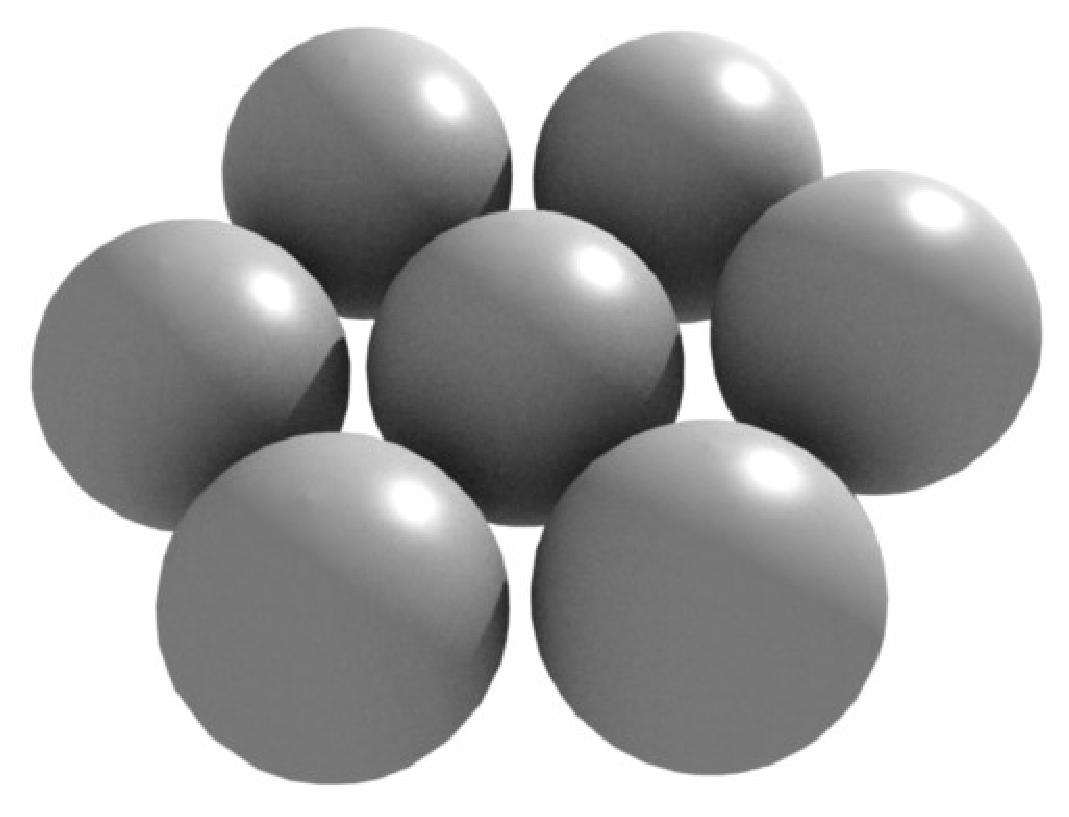
\includegraphics[width=100mm]{images/willitblend.eps}
		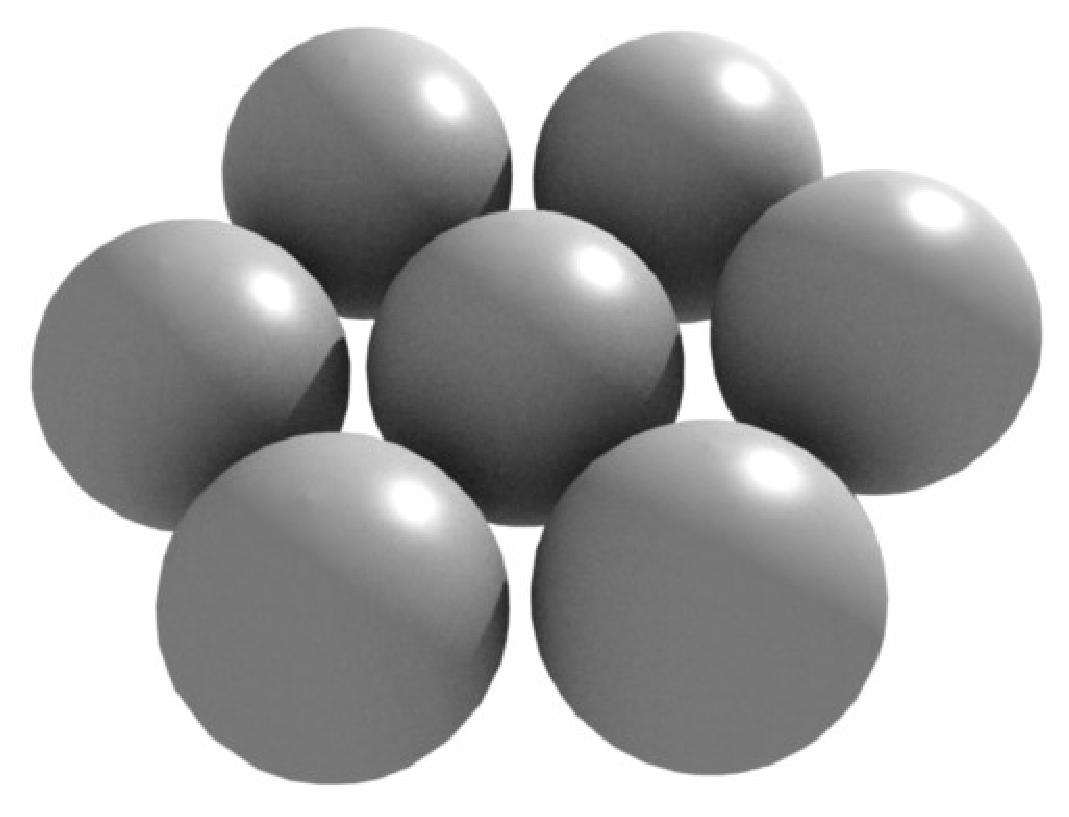
\includegraphics[width=50mm]{images/willitblend.eps}
	\end{figure}
	[image in which the gold particles are modeled as packed spheres]	
	
	The approximate ligand length is 2${\mu}m$ for Au$_{314}$ and approximately 1${\mu}m$ for Au$_{25}$.
	The approximate size of the colloidal gold particles are 2.5${\mu}m$ for Au$_{314}$ and 1${\mu}m$ for Au$_{25}$.
	Making the assumption that these particles can be modeled as spheres of radius 3${\mu}m$ for Au$_{314}$ and 1.5${\mu}m$ for Au$_{25}$ leads to a relative density of 4 nanoparticles of Au$_{25}$ per nanoparticle of Au$_{314}$, which yields an approximate density of 100/314.
	
	At the first order, three times more layers of Au$_{25}$ should therefore be deposited to yield an equivalent gold mass to the Au$_{314}$ film.
	
	In real application, thermolysis of much more than 8 layers of a film will result in defects of significant density to affect the production of our nanoislands of interest.
	It is therefore better to use larger Au$_{314}$ particles instead of many layers of Au$_{25}$.


	\subsection{How to Evaluate the Reproducibility of Nano-Island Samples}
	The effectiveness of our process control can be evaluated through direct and indirect measurement of the uniformity of the resulting nano-islands.  
	Nano-island size and uniformity can be measured directly through atomic force microscope (AFM) images.  
	Scanning electron microscope (SEM) images may also be used to evaluate size and uniformity, but these images lack resolution to evaluate sizes below {\bf $50nm$ (TBR)}.  
	Spectral measurements of the nano-island samples will show absorption features which can be used, along with the direct measurements, to indirectly indicate the uniformity of the size distribution of the nano-islands.
	
	\begin{quote}
		Because there is inherent heterogeneity among individual nanoparticles, each LSPR spectrum is different, revealing the true distribution of resonance wavelengths (20, 98).		
		(www.annualreviews.org - Localized Plasmon Spectroscopy
	271)
	\end{quote}


	\subsection{Size and Shape Distributions and Phonon Absorption Features}
	The uniformity of the size and shape is expected to correlate with the width of the absorption feature of the resulting sample.
	A wider distribution of sizes and shapes is expected to produce a broader absorption peak, while a narrower distribution of nanoisland sizes about the average size is expected to produce a sharper absorption feature.
	This relationship is predicted analytically because identical islands should absorb identically (neglecting second-order effects), producing a maximized peak.  
	Differences among the islands will create phonons that are offset by some amount from the peak wavelength, resulting in a lower and broader peak.
	
		
	
	% This absorption peak should be tested if i can measure the distribution of size features along with the spectral properties.
	% Now who has the specral analysis setup?  (YS SHON) 
	% A review article referenced by Joshi thesis may identify the relationship between peak sharpness and size distribution.  
	% This relation is intuitive to me and to Chuhee, but would benefit from a reference.
	
	\subsection{Procedure for Preparing Gold Slides}
	
	\subsubsection{Preparation of Gold Nanoparticle Solution}
	The preparation of the gold nanoparticle solution requires about a week of preparation to yield the 10 mL of Au$_{314}$.
	

	\subsubsection{Layering the Samples}
	To deposit the self-assembling multilayers on a glass electrode, the following steps are 
	\begin{itemize}
		\item First Day
		\begin{itemize}
			\item An aqueous solution of poly(allylamine hydrochloride) (PAH) is prepared, adding 10mg PAH to 10mL nanopure water, for use on Day Three.
			\item 1.0mL methanol is added to 0.1mL triethyl 3-mercaptopropylsilane in a 5mL vial.
			\item 0.1mL of nanopure water is added to the solution.  (The triethyl 3-mercaptopropylsilane will react with the water and the solution becomes cloudy).
			
			\item The IDE is placed in the solution for 24 hours.
			\item \emph{Note}: it is important not to leave the IDE for more than 24 hours, or the IDE will acquire a thick deposited coating.
		\end{itemize}
		\item Second Day
		\begin{itemize}
			\item The IDEs are placed in clean 5mL vials.
			\item Methanol is added to the vials and the samples are sonicated in an ultrasonic bath.
			\item The methanol wash is removed, and the washing process is repeated 2 more times.
			\item After the third ultrasonic wash, the samples are gently dried under a stream of nitrogen gas or air.
			\item After drying, gold nanoparticle solution is added to each vials, enough to cover the IDE.
			\item The IDEs are left in the nanoparticle solution overnight.
		\end{itemize}
		\item Third Day
		\begin{itemize}
			\item A work station is prepared with an ultrasonic bath, Pasteur pipettes, nanopure water, ethanol, PAH solution, and several spare 20mL vials for containing waste or re-used liquids.
			\item for layer = 2:10 
			\begin{itemize}
				\item The gold nanoparticle solution is removed from each vial using Pipette A and placed in a 20mL vial for reuse.
				\item A washing solution of nanopure water (Au$_{25}$) or ethanol (Au$_{314}$) is added to each vial using Pipette A, and the vials are placed in an ultrasonic bath.
					\subitem Washing the IDE by inverting the vials is not recommended, as this breaks bonding wires.  An ultrasonic bath prevents damage to the wire bonds.
				\item If the nanoparticle solution is Au$_{314}$, the ethanol is removed with Pipette A, nanopure water added, and the vials are again placed in the ultrasonic bath.
				\item The nanopure water is removed from the vial (for Au$_{314}$ and Au$_{25}$) using Pipette A.
				\item The PAH solution is added to each vial using Pipette B and the vials are left to stand for 5 minutes.
				\item The PAH solution is removed from the vials using Pipette B,  nanopure water is added with Pipette B, the vials are placed in an ultrasonic bath, and the nanopure water is removed using Pipette B.
				\item If Au$_{314}$, then add ethanol using Pipette A and place the vial once more into the ultrasonic bath, and the ethanol is removed with Pipette A.
				\item If this layer is not the last layer, the Au$_{314}$ or Au$_{25}$) solution is added to the vials using Pipette A, and the vials are left to stand for 5 minutes.
			\end{itemize}
			\item end for loop (next layer)
			\item The IDEs are gently dried under a stream of nitrogen gas or air, and placed in a vacuum desiccator in the dark, for storage.
		\end{itemize}
	\end{itemize}

	\subsection{Bonding and Baking}
	
	\subsection{The importance of accurate temperature measurement}
	Use of multiple thermocouples (Figure "oven_tc") to measure oven temperature during very rapid heating showed large temperature gradients within the oven, and that the glass slides on which the samples are mounted slow the heating of the sample.

	Three thermocouples were used to measure oven temperature.  
	The oven has a heavy gauge K-type thermocouple at the top of the oven (tc3 in figure N).  
	A bare 10 mil ($254{\mu}m$) thermocouple (tc2 in figure N) was situated near the bottom of the oven.  
	A third thermocouple (tc1 in figure N) was attached to a glass microscope slide with a dab of silver epoxy and placed next to the sample.
	
	The IDE sample is responsive to temperature, and a bare IDE should show the same impedance during (fast) heating as it shows during (slow) cooling (Figure "logR_vs_t1_and_t3").  
	If the temperature measured by a thermocouple results poor overlap of the IDE impedance on the heating and cooling phases, a temperature error can be inferred.
	In this way the bare slide can serve as a fourth temperature-sensitive device to confirm that the "sample temperature" inferred from the thermocouple temperature measurements accurately tracks temperature.  
	
	The glass slide thermocouple placed next to the sample under test (DUT) was shown to best track the DUT temperature.  The glass slide was also used to close the loop of the oven PID for all tests in Spring 2012.  However, because the glass is slower to heat than the air, it can cause a situation in which the oven overheats.  The bare IDE may be a better candidate for the oven PID control, as it measures the air temperature in the oven.  
	
	The oven PID controller creates a closed-loop temperature control system, using a single thermocouple to measure the oven temperature, and a solid-state relay to turn the oven on and off. 
	In the modified temperature controller, any thermocouple can be used in the PID controller, and we selected a thermocouple mounted to a glass slide by silver epoxy, since it better tracks the temperature of the IDE sample.
	It was discovered that the glass slide IDE lags behind the temperature at the top of the oven by as much as $200^{\circ}C$ during fast heating of $30^{\circ}C/min$ (Figure "plot_tc3_vs_tc1").  The build-up of heat and the lag of the glass TC resulted in an overheating of the oven when there is no additional safety measures.  A safety measure was introduced into the oven controller code to turn off the heat if any TC measured greater than $+50^{\circ}C$ from the oven setpoint.
	
	
	
	
	
	\section{Electron Transport Measurement using Complex Impedance}
	A four-point impedance measurement measures complex impedance of the IDE sample under test (device under test, or DUT).  Impedance measurements follow a temperature dependence derived from models of electron transport under an AC potential.  Complex impedance and temperature measurements are used to solve electron mobility under the AC electron transport model detailed below.  Temperature measurements were limited to those measurements taken during cool-down of the DUT, since temperature measurements during fast heating of the sample carry very large errors.  Measurements of impedance over temperature during cool-down (FIGURE "cooldown_residuals") were identical within uncertainties for the Au$_25$ sample (JD04) and a bare IDE sample (JD05), and electron mobility will be identical.  Electron mobility calculated for the Au$_25$ (JD04) sample was ${\epsilon\over{k}} = 1.1e+04 K$, $\epsilon = 0.96 eV$.
		
	\subsection{Introduction: Measurement of Complex Impedance} 
	DC resistance measurements of the electrode show only its insulating properties, as the glass substrate is a poor conductor and the IDE is a weak capacitor, so AC resistance is measured.
	AC resistance in the IDE samples follows the temperature-dependent electron mobility.
	
	\begin{equation}
		R = R_0 \cdot e^{\epsilon\over{k \cdot T}}
		\label{eq:emobility}
	\end{equation}
	
	This equation can be rearranged into a linear equation to solve for $\epsilon$.
	
	\begin{equation}
		ln(R) = {\epsilon\over{k}} {1\over{T}} - ln(R_0)
		\label{eq:solve_emobility}
	\end{equation}
	
	${\epsilon\over{k}}$ and $ln(R_0$ are found by least-squared fit of the linear portion of the data.
	
	\begin{figure}
	
	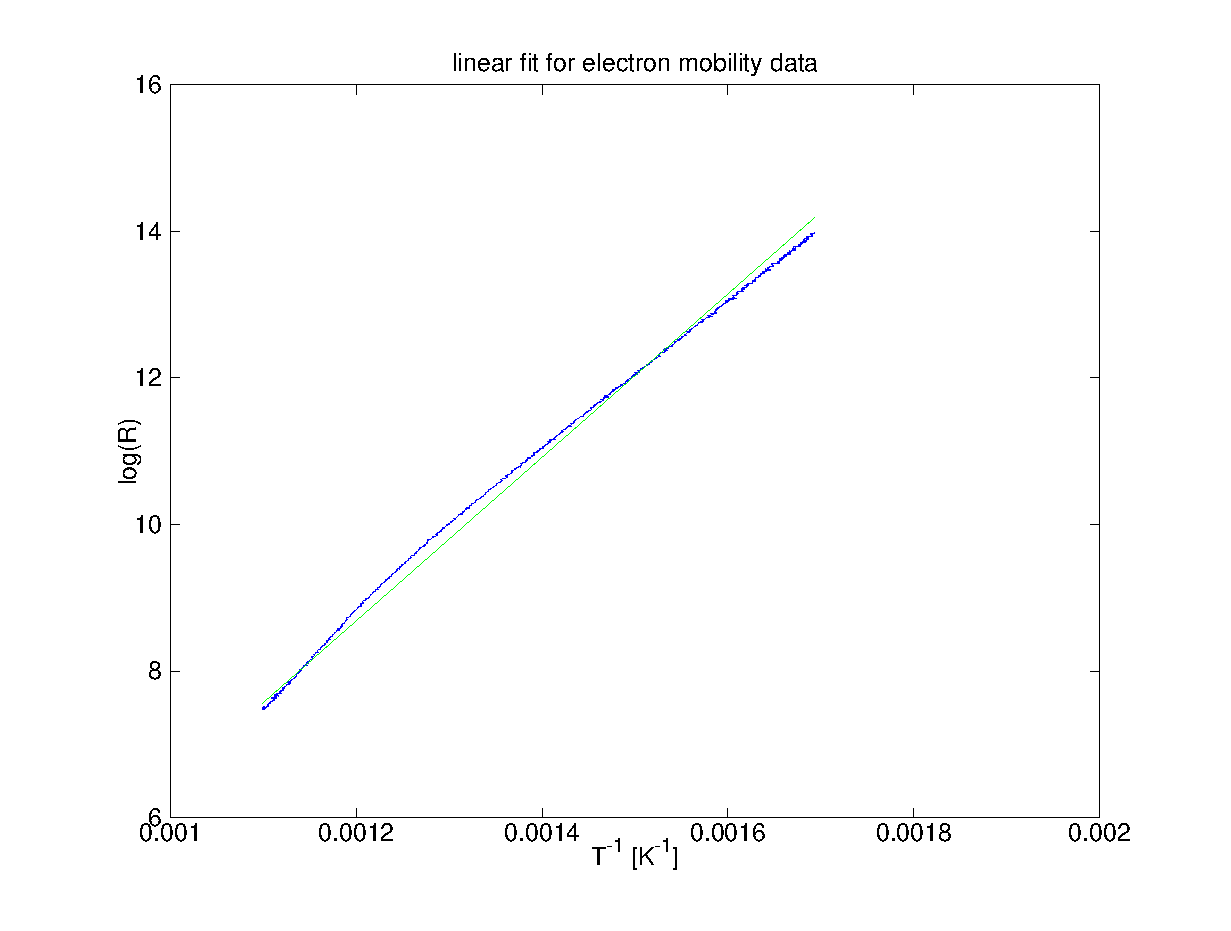
\includegraphics[scale=0.4]{images/electron_mobility.eps} 
	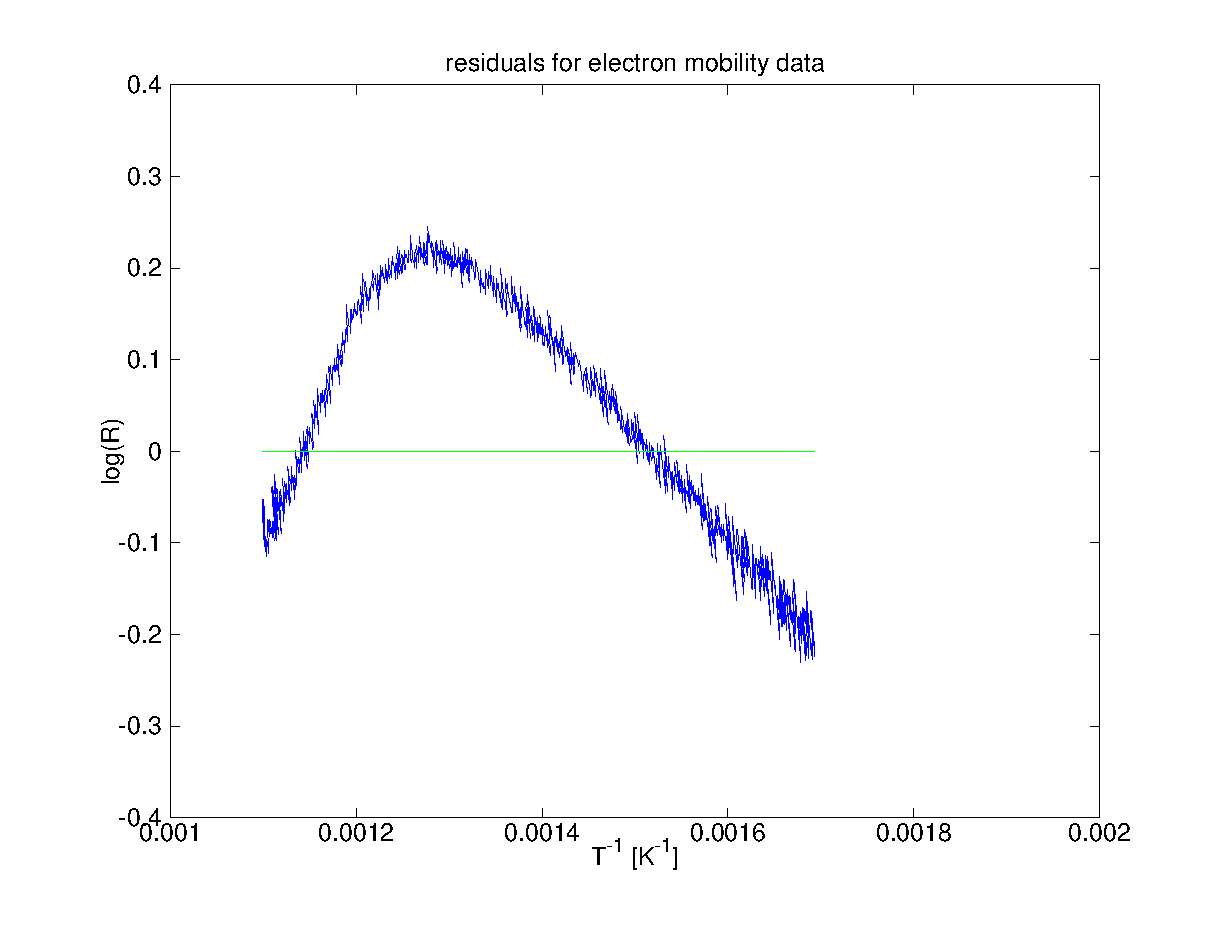
\includegraphics[scale=0.4]{images/electron_mobility_residual.eps}
	\label{f:emobility}
	\caption{During cool-down of the sample, the impedance versus temperature measurements are well-sampled, and can be used to solve for electron mobility.  ${\epsilon\over{k}} = 1.1e+04 K$, $\epsilon = 0.96 eV$, $R_0 = 9.1e-3\Omega$.  Error bars are needed, and will have magnitude at least proportional to the fit residuals.}
	\end{figure}
	The temperature range observed is between $295K$ and $900K$, 
	
	Sample resistance (a parallel AC resistance) is typically high for the sample under test, this resistance changes when the sample is heated and the polymers are burned off.  

	The resistance $R_p$ of a high-resistance sample can be measured from the complex impedance $(Z,\theta)$ by Equation ~\ref{eq:R_p}.  Use of the parallel resistance $R_p$ is justified at high sample resistance because the series resistance $R_s$ of the test leads and contacts are orders of magnitude smaller.
	
	\begin{equation}
		R_p = {{Z} \over {cos({\theta})}}
		\label{eq:R_p}
	\end{equation}
	
	Typical values for complex impedance measured by the auto-balancing bridge method via an Agilent 82XX LCR meter are as follows.
	
	\begin{equation}
		\left( Z,\theta,\nu,T \right) = \left( 15 M\Omega, -89.9^\circ, 1kHz, 22^{\circ}C \right)
	\end{equation}
	\begin{equation}
		\left( Z, \theta, \nu, T \right) = \left( 800 k\Omega, -88^\circ, 45kHz, 22^{\circ}C \right)
	\end{equation}
	
	This result shows that the $R_p$ ``resistance'' component (which is $Z$ divided by $cos(-89^\circ)$) is immeasurably high at low frequencies and low temperature.  It is only at higher temperatures that $R_p$ drops to the measurable range, and this occurs at about $250^{\circ}C$ when the impedance phase angle $\theta$ drops from $-89.9^\circ$ towards $0.1^\circ$.
	
	During the burn-off of the polymers, the parallel resistance may drop to under 100 ohms, which requires a four-point measurement to compensate for the series resistance test lead impedance.
	A four-point measurement is necessary because the test leads have been reported (AD5933) to have up to kilo-ohm impedance when measuring low sample resistance.


\clearpage
\bibliography{thesis_draft}
\bibliographystyle{plain}


\end{document}

%% ******************************************************************
%% The following is some template materials -- equations and figures.
\documentclass[aps,prl,twocolumn,oneside,showkeys,floatfix]{revtex4-1}
\newcommand{\BibTeX}{{\sc Bib}\TeX}
\usepackage{graphicx}
\usepackage{listings}

\newbox\bwk\edef\tempd#1pt{#1\string p\string t}\tempd\def\nbextr#1pt{#1}
\def\npts#1{\expandafter\nbextr\the#1\space}
\def\ttwplink#1#2{\special{ps:1 0 0 setrgbcolor}#2\special{ps:0 0 0 setrgbcolor}\setbox\bwk=\hbox{#2}\special{ps:( linkto #1)\space\npts{\wd\bwk} \npts{\dp\bwk} -\npts{\ht\bwk} true\space Cpos}}
        \begin{equation}
        \nu_{\mathtt{Larmor}} = {{\Delta E} \over{ 2 \pi \hbar}} = {{2 B \cdot \mu_{\mathtt{proton}}} \over{2 \pi \hbar}}
        \end{equation}

        \author{John \surname{Donovan}}
        \affiliation{CSULB}
        \begin{abstract}
                \begin{description}
                        \item[Background] This part would describe the
                        context needed to understand what the paper
                        is about.
                        \item[Purpose] This part would state the purpose
                        of the present paper.
                        \item[Method] This part describe the methods
                        used in the paper.
                        \item[Results] This part would summarize the
                        results.
                        \item[Conclusions] This part would state the
                        conclusions of the paper.
                \end{description}
        \end{abstract}
        \keywords{nano,nano-islands,thin films}
        \maketitle
        Written in \LaTeX\ with TexMaker.


\begin{figure}
\includegraphics[scale=0.5]{BField_Set1.eps} \label{BSet1}
\caption{The magnetic field (in MHz resonance frequency) measured.  Set 1 did not include many measurements of the most uniform part of the field.}
\end{figure}

\clearpage
\begin{widetext}
\section{Appendix}
\subsection{Spin Echo Peak-Finder Algorithm in Matlab}
\lstset{language=Matlab, basicstyle=\footnotesize, numbers=left, captionpos=t, breaklines=true, caption=find\_spin\_echo() locates the pulse maxima in a spin-echo pulse train, label=T2 Pulse Train, frame=shadowbox}
\lstset{basicstyle=\small\ttfamily, basewidth=0.51em}
\lstinputlisting{../find_pulse_train.m}
\end{widetext}

%% *******  END OF TEMPLATE MATERIALS  ******************************
%% ******************************************************************

%% *******  Draft Material *******
